\documentclass{ctexart}
\usepackage[backend=biber]{biblatex}
\usepackage{amsmath, amsfonts, amsthm}
\usepackage{siunitx}
\usepackage{braket}
\usepackage{asymptote}
\usepackage{enumitem}
\usepackage{xcolor}
\usepackage{subcaption}
\usepackage{hyperref}

\numberwithin{equation}{subsection}
\newtheorem{theorem}{定理}[section]
\newtheorem{lemma}[theorem]{引理}
\newtheorem{proposition}[theorem]{命题}
\newtheorem*{corollary}{推论}
\theoremstyle{definition}
\newtheorem{definition}{定义}[section]

\DeclareSIUnit\cell{cell}
\DeclareSIUnit\calUnit{cal}

\title{固体物理学学习汇报}
\author{***REMOVED***\thanks{***REMOVED***}}
\addbibresource{references.bib}

\begin{document}
\maketitle
\tableofcontents
\clearpage

\section{基础知识}

本节主要介绍固体物理课程上学习到的各种基础知识,这些知识将用于支撑对半导体材料的性质的计算。

\subsection{代数学基本知识}

我们首先介绍几个常用的代数学定义。

\begin{definition}
    群(group)是装备有二元关系$\cdot$的非空集合$G$构成的有序二元组$(G, +)$,该二元关系满足:
    \begin{enumerate}[nosep]
        \item 结合性,即
            $$x\cdot ( y \cdot z) = (x \cdot y) \cdot z, \; \forall x,y,z \in G$$
        \item 存在单位元,即
            $$\exists e \in G, \text{s.t. } x \cdot e = e\cdot x = x, \; \forall x \in G$$
        \item 存在逆元,即
            $$\forall x \in G, \exists y \in G, \text{s.t. } x \cdot y = y \cdot x = e$$
    \end{enumerate}
    若该二元关系还是可交换的,即
    $$x \cdot y = y \cdot x, \; \forall x, y \in G$$
    那么这个群称为交换的,或阿贝尔的(abelian)。
\end{definition}

可以证明,群的单位元和每个元素的逆元都是唯一的。

\begin{definition}
    格点(lattice)是向量空间$\mathbb R^n$的有限生成阿贝尔子群(finitely-generated abelian subgroup),满足
    $$\Lambda = \left\{ \sum_{i=1}^n a_i v_i \; \middle\vert\; a_i \in \mathbb Z \right\}$$
    其中$v_i$是向量空间$\mathbb R^n$的基底。对偶空间中的格点称为该格点的对偶格点(dual lattice),满足
    $$\Lambda^* = \left\{ v^* \in \mathbb R^n \; \middle\vert \; v^* \cdot v \in \mathbb Z ,\, \forall v \in \Lambda \right\}$$
    数学上可认为对偶格点中的元素在对偶空间${{\mathbb{R}}^n}^*$中。
\end{definition}

不同的基底可以生成相同的格点,然而从格点还原计算基底是困难的。
但是这些基底的行列式的绝对值,即一个格点对应的面积或体积,永远是一致的。

\subsection{晶格对称性的数学表述}

晶体中所有原子的排列服从一定的规律,这种规则的排列称为晶体的晶格。
晶格的特点是具有周期性,无论具有什么样的结构,总是可以看作是由某平行六面体划出的单元沿着三条边的方向重复排列而成的。
这种重复的排列在数学上可由格点表示。

\begin{definition}
    晶体的最小周期单元称为该晶格的原胞(primitive cell),其棱张成的格点称为晶体的布拉伐格点(Bravais lattice),这一格点的基底,即原胞的棱,习惯上用$a_i$表示。
\end{definition}

若布拉伐格点已经给出,则可在其中圈出晶格的原胞。
首先,选定格点中的一点,然后将布拉伐格点中与该点相邻的点以线段相连,取连线段的垂直平分线,圈出的凸多边形即为一个原胞,这种原胞称为维格纳-赛兹原胞(Wigner–Seitz cell)。

晶体的周期性表明,晶体中任何具有物理意义的量总是满足关于晶格的平移对称性。

\begin{proposition}
    设$V: \mathbb R^{2,3} \to K$为晶格中一物理量,则
    $$V(x) = V(x + l), \; \forall l \in \Lambda$$
    其中$\Lambda$是是晶格的布拉伐格点。
\end{proposition}

在考虑了晶胞的平移对称性后,我们还希望考虑其旋转对称性,而这在数学上通常通过群来完成。

\begin{definition}
    点群(point group)是欧几里得空间中具有共同不动点的等距变换构成的群,习惯上这一共同的不动点选取在欧几里得空间的原点处。这些群是正交群$O(n)$的子群。
\end{definition}

以二维空间为例,所有$n$次旋转,即每次转动$\frac{2\pi}{n}$角度的旋转,均可构成一个点群,这些点群表征了二维平面上的中心对称,记作$C_n$。
这些群同构于$Z_n$。

若同时考虑晶格的旋转对称性和平移对称性,则并非所有的旋转均可与平移兼容,所有这些兼容的仿射变换,即同时包括平移和旋转的变换,又构成一个群,称为空间群。

\begin{definition}
    三维空间中晶体中可能出现的仿射变换组成的群称为空间群(space group)。
    二维空间中这样的群称为壁纸群(wallpaper group)或平面群(plane group)。
\end{definition}

当同时考虑平移和旋转对称性时,能够发现,并非所有平移和旋转变换均可兼容。

\begin{theorem}
    (晶体学限制定理)
    在二维和三维的格点中,能够出现的表示旋转的点群的阶数,能且仅能是$1,2,3,4,6$其中之一。
\end{theorem}

\begin{proof}
    课上给出了一个几何的证明,此处利用变换的迹给出另一个证明。
    我们知道,矩阵的迹是相似不变的,即任意选择空间的基底,同一变换在不同基底之下的矩阵表示的迹是一致的。因此,在格点空间中,由于变换一定将整数坐标映射到整数坐标,因此一定可以选择恰当的基底,使得矩阵的迹是整数。而正交矩阵的迹与旋转角度有关:
    $$\mathrm{tr}(O) = 1 - 2 \cos \theta \in \mathbb Z \implies \cos \theta = 0, \pm 1, \pm \frac{1}{2}.$$
    从而旋转角度仅能为
    $$\theta = 0^\circ, 60^\circ, 90^\circ, 120^\circ, 180^\circ. \qedhere$$
\end{proof}

三维空间中的点群可分为七个大类,其中每一类均有无限个群,然而由于晶体学限制定理,可能在三维晶体中出现的仅有32种。
这三十二种点群又分为七种晶系和十四种布拉伐格点,进而产生230中空间群。
这些空间群就表示了晶体所有可能的结构。

\subsection{倒易空间}

在研究薛定谔方程时,我们通过傅里叶变换将实空间中的粒子变换到傅里叶空间中进行研究。
在晶体中,我们也可以利用傅里叶变换,在对偶空间中研究晶体的性质,这一点尤其重要,因为我们知道,电磁波的衍射与傅里叶变换有密切的关系。

\begin{definition}
    晶体的布拉伐格点的对偶格点,称为该晶体的倒易格点(Reciprocal lattice),简称倒格点。
\end{definition}

\begin{proposition}
    三维空间中倒格点的一组基底是
    $$b_1 = \frac{a_2 \times a_3}{a_1 \cdot (a_2 \times a_3)}, b_2 = \frac{a_3 \times a_1}{a_2 \cdot (a_3 \times a_1)}, b_3 = \frac{a_1 \times a_2}{a_3 \cdot (a_1 \times a_2)},$$
    这是倒格点最常用的一组基底。这组基底满足正交性,即
    $$a_i b_j = \delta_{ij}.$$
\end{proposition}

基底的正交性容易验证,此处给出该基底确实为对偶格点基底的证明。

\begin{proof}
    首先,显然$b_i$是线性独立的,因此其必是$\mathbb R^3$的一组基底,因此对偶格点中的所有向量均可由其表出:
    $$v^* = h_1 b_1 + h_2 b_2 + h_3 b_3, \; \forall v^* \in \Lambda^*.$$
    仅需证明$h_i$均为整数即可。
    根据对偶格点的定义,有$v^* \cdot a_1\in \mathbb Z$,
    从而
    $$(h_1 b_1 + h_2 b_2 + h_3 b_3) a_1 = h_1 \in \mathbb Z$$
    其他两轴同理。
    因此,$b_i$确为对偶格点的基底。
\end{proof}

在物理中,我们倾向于使用以下基底:
$$
b_1 = 2\pi \frac{a_2 \times a_3}{a_1 \cdot (a_2 \times a_3)}, 
b_2 = 2\pi \frac{a_3 \times a_1}{a_2 \cdot (a_3 \times a_1)}, 
b_3 = 2\pi \frac{a_1 \times a_2}{a_3 \cdot (a_1 \times a_2)}
$$
这种表示方式不符合数学上的对偶格点的要求,但是在研究傅里叶展开时更加有用,其正交性也变为$a_i b_j = 2\pi \delta_{ij}$

倒易空间的重要性由以下命题揭示。
\begin{proposition}
    若某一函数在正空间中具有周期性,即
    $$f(r) = f(r + R), \; \forall R \in \Lambda,$$
    则其傅里叶变换在倒空间中具有相同的周期性,即
    $$F(k) = F(k + G), \; \forall G \in \Lambda^*.$$
\end{proposition}

\begin{proof}
    考虑周期函数的傅里叶变换:
    $$F(k) = \iiint_{V_\text{晶胞}} f(r) \exp[-ik\cdot r] \,\mathrm d V$$
    计算$F(k + G)$:
    $$F(k+G) = \iiint_{V_\text{晶胞}} f(r) \exp[-i(k+G)\cdot r] \, \mathrm d V$$
    现在,根据倒空间的基底,注意到$G \cdot r \in 2 \pi \mathbb Z$,
    从而
    $$F(k+G) = \iiint_{V_\text{晶胞}} f(r) \exp[-ik\cdot r] \exp[-2i\pi] = F(k). \qedhere$$
\end{proof}

这意味着,晶体的周期性不仅存在于实空间——即位置空间——中,也存在于傅里叶变换之后的空间——即动量空间——中。
因此,晶体的晶胞也不仅仅存在于一个看得见、摸得着的实际的空间中,也存在于动量空间中。
特别地,倒空间中的维格纳-赛兹原胞称为(第一)布里渊区。


\section{晶体计算}

本节主要介绍利用 Material Studio 2020\footnote{Material Studio 8在 Windows 11 上不能正常运行。} 对硅晶体的各项属性进行模拟计算的操作步骤与结果。

\subsection{硅晶体的构建}

硅晶体是常见的本征半导体之一,也是进行掺杂来构造其他半导体的典型基体。
其晶胞为金刚石型面心立方结构,皮尔逊表示为 cF8,室温下的晶胞参数为$a = \qty{543.0986}{\pico\metre}$\cite{selectedvalues2018john,Grazulis2009,Downs2003}。
该晶胞对应的空间群为$\mathrm{Fd\overline{3}M}$,表示面心布拉伐格点(F)、金刚石型平移对称(d)、旋转反演角为$\frac{\ang{360}}{3}=\ang{120}$、镜像面与转轴垂直(M)。
图~\ref{fig:silicon-cell}~展示了硅晶体的晶胞与原胞,其中晶格参数即为红色立方体的边长。

\begin{figure}[ht!]
    \centering
    \begin{asy}
        include "./silicon-cell.asy";
    \end{asy}
    \caption{硅晶体的晶胞(红色)与原胞(蓝色)}\label{fig:silicon-cell}
\end{figure}

为在 Material Studio 中为该分子建模,首先新建原子结构文件(3D Atomistic),然后在下拉菜单中选择构造(Build)、晶体(Crystal)、构造晶体(Build crystal)。
在新对话框中输入晶体的空间群,然后输入晶格参数,即可完成晶胞的构建。
然后,向其中加入原子,选择构造(Build)、添加原子(Add Atoms)并填入原子的元素符号,即可在晶胞中填充原子。
图~\ref{fig:ms-cells}展示了 Material Studio 中构建的晶体。

\begin{figure}
    \centering
    \begin{subfigure}[c]{0.4\linewidth}
        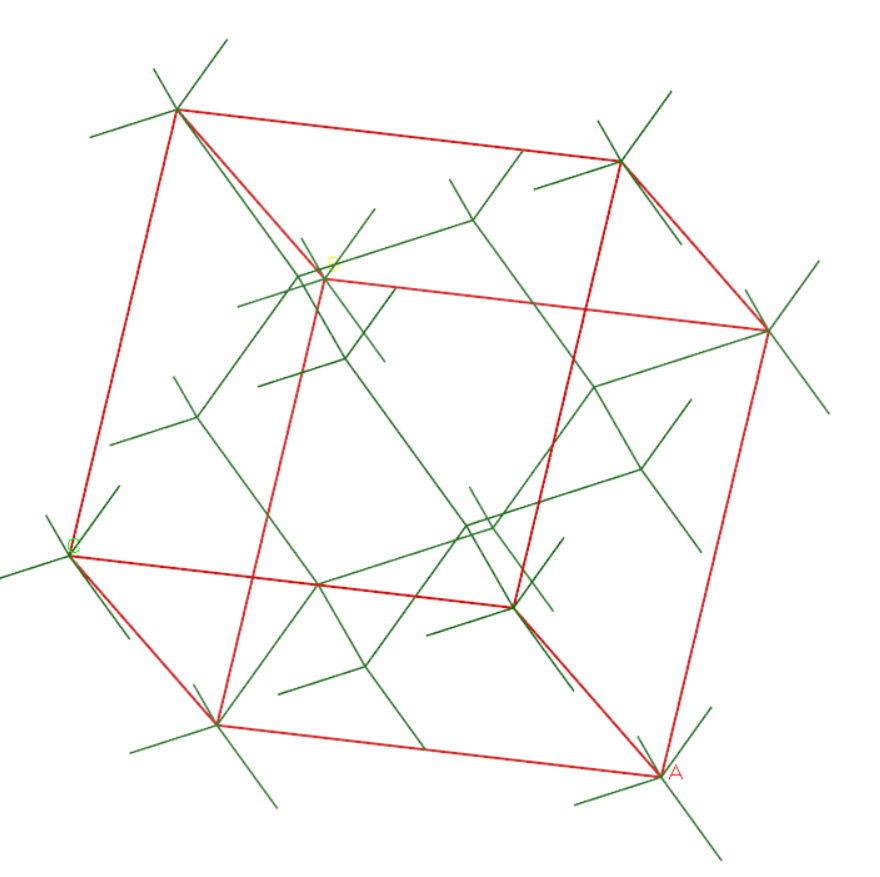
\includegraphics[width=\linewidth]{screenshots/unit-cell.png}
    \end{subfigure}
    \begin{subfigure}[c]{0.4\linewidth}
        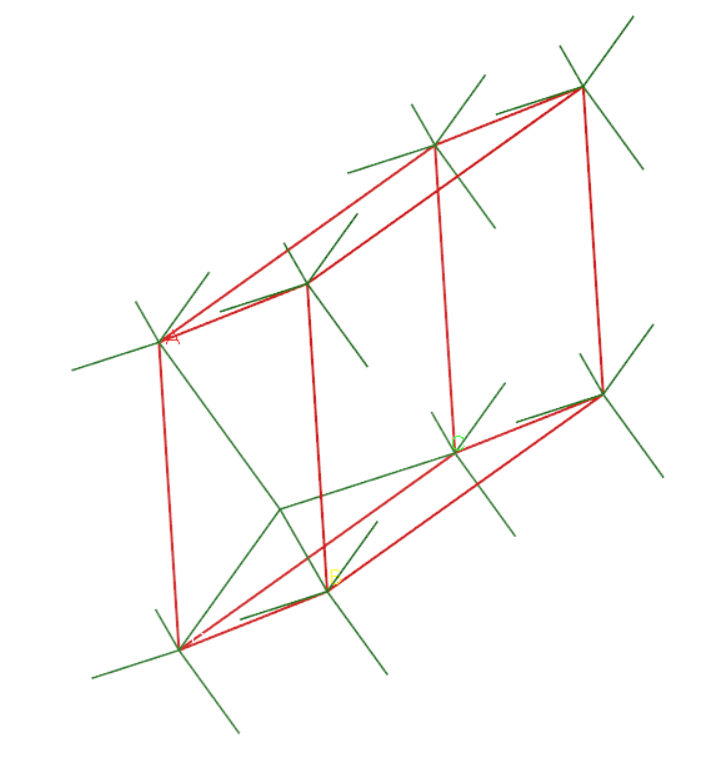
\includegraphics[width=\linewidth]{screenshots/primitve-cell.png}
    \end{subfigure}
    \caption{Material Studio 中晶体的晶胞与原胞}\label{fig:ms-cells}
\end{figure}

\subsection{布里渊区与 K 路径}

我们考虑金刚石型晶体——或更一般的,面心立方晶体的布里渊区的结构。

\begin{proposition}
    面心立方晶体的(第一)布里渊区是倒空间中的截角八面体(truncated octahedron),即从正八面体的角上截去六个相同的四棱锥形成的多面体,如图~\ref{fig:truncated-octahedron}所示。
\end{proposition}

\begin{figure}[ht!]
    \centering
    \begin{asy}
    include "./truncated-octahedron.asy";
    \end{asy}
    \caption{倒空间中的截角八面体,从四根轴中任取三根即可组成倒空间的基底。}
    \label{fig:truncated-octahedron}
\end{figure}

\begin{proof}
    不妨设面心立方晶胞的边长为$\frac{2}{\pi}$,考虑正空间中的原胞产生的格点的基底
    \begin{equation}
        a_1 = (\frac{1}{\pi}, \frac{1}{\pi}, 0), \; a_2 = (\frac{1}{\pi}, 0, \frac{1}{\pi}), \; a_3 = (0, \frac{1}{\pi}, \frac{1}{\pi}).
    \end{equation}
    对应的倒空间基底自然为
    \begin{equation}
        b_1 =  (1, 1, -1), b_2 = (1, -1, 1), b_3 = (- 1, 1, 1).
    \end{equation}
    这三个基底向量和$(-1,-1,-1)$将倒空间分为对称的四个部分。
    由于原胞的基底不正交,倒空间的基底也不正交,其立体夹角为
    \begin{equation}
        \phi = \arccos \frac{b_1 \cdot b_2}{\Vert b_1 \Vert \cdot \Vert b_2 \Vert} \approx \ang{109.47}.
    \end{equation}
    我们现在仅考虑一个卦限中的情况,其他情况可容易地根据对称性推出,考虑与原点紧邻的七个格点,首先在倒空间基底中写出其坐标:
    \begin{equation}
        \begin{aligned}
            A(1, 0, 0), B(0, 1, 0), C(0, 0, 1), D(1, 1, 1) \\
            E(1, 1, 0), F(1, 0, 1), G(0, 1, 1), 
        \end{aligned}
    \end{equation}
    然后回到笛卡尔坐标系中,首先注意$A, B, C, D$:
    \begin{equation}
        A' (1, 1, -1), B' (1, -1, 1), C'(-1, 1, 1), D'(1, 1, 1),
    \end{equation}
    从原点到这四个点的连线的垂直平分面截成了正八面体的一部分,而剩下三个点的垂直平分面则从这个正八面体中截除了全等的三个四棱锥。
\end{proof}

为在 Material Studio 中给出第一布里渊区的形状与自动计算的 K 路径,首先选择构建(Build)、对称性(Symmetry)、原胞(Primitive Cell)来展示晶胞的原胞视图。
然后选择工具(Tools)、布里渊区路径(Brillouin Zone Path)即可生成K路径。
图~\ref{ref:ms-brillouin-zone}展示了上述操作的结果。

\begin{figure}[ht!]
    \centering
    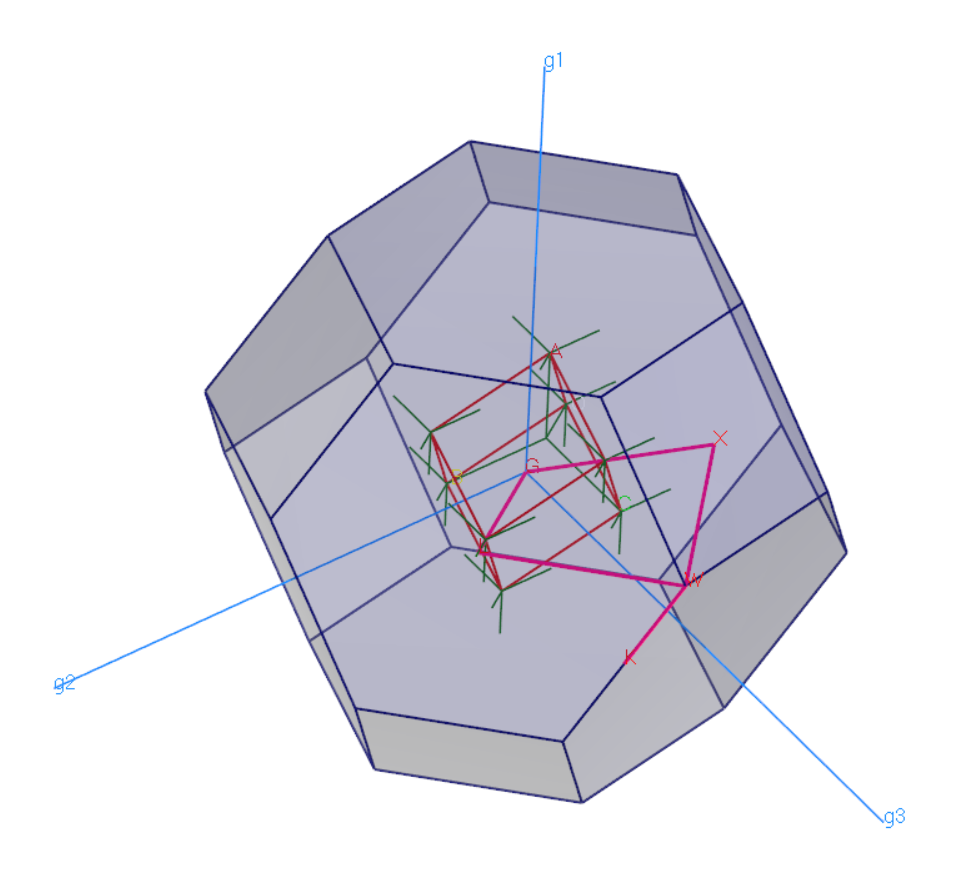
\includegraphics[width=0.8\linewidth]{screenshots/reciprocal.png}
    \caption{Material Studio 中的布里渊区与路径。}
    \label{ref:ms-brillouin-zone}
\end{figure}

\subsection{计算能带}

最后,我们以能带为例展示在 Material Studio 中计算物质性质的步骤。
首先,选择计算使用的软件包,此处我们选择 CASTEP 包。

在保持最初的原子结构文件打开的情况下,从菜单栏中选择 CASTEP 计算(CASTEP Tools \verb|->| Calculation)。
根据 CASTEP 包的说明,我们首先需要计算能量,然后才能给出晶体的属性。
在“任务”(Task)下拉菜单中选择“能量”(Energy),计算品质选择“精细”(Fine),取消勾选“金属”(Metallic)选项,其他设置保持默认,然后在“属性”(Properties)选项卡中勾选需要的“属性”,单击运行(Run)开始计算。
此处我们选择的属性有“能带结构”(Band structure)、“态密度”(Density of states)和“声子”(Phonons),为计算声子,必须选择保范数的赝势。
在作业(Jobs)窗口中观察,等待任务完成。

任务完成以后,项目中会生成多种文件,包括记录晶体结构的 \verb|*.xsd| 文件和计算参数的 \verb|*.param| 文件、输出的 \verb|status.txt| 日志文件、计算中使用的参考文献生成的 \verb|*.bib| 文件以及计算的结果。

首先考虑 \verb|status.txt| 文件,该文件包括以下内容:
\begin{enumerate}
    \item 标头,包括进行计算的时间、计算机名和软件包信息等;
    \item 结果概况,包括原子信息、使用的赝势、收敛迭代数(\texttt{Converged in 54 iterations ...})和本征值等;
    \item 配置信息,此处基本是 Material Studio 默认的配置;
    \item 计算参数,包括原胞的各种参数、原子的位置和对称性等;
    \item 尾部,包括计算使用的时间。
\end{enumerate}

为分析能带结构,需选择“分析”(Analysis)选项并选择“能带结构”(Band structure),勾选“能带密度”(DOS)并确认即可画图,图~\ref{fig:si-band-structure-castep}展示了CASTEP 计算的能带的结构。

\begin{figure}[ht!]
    \centering
    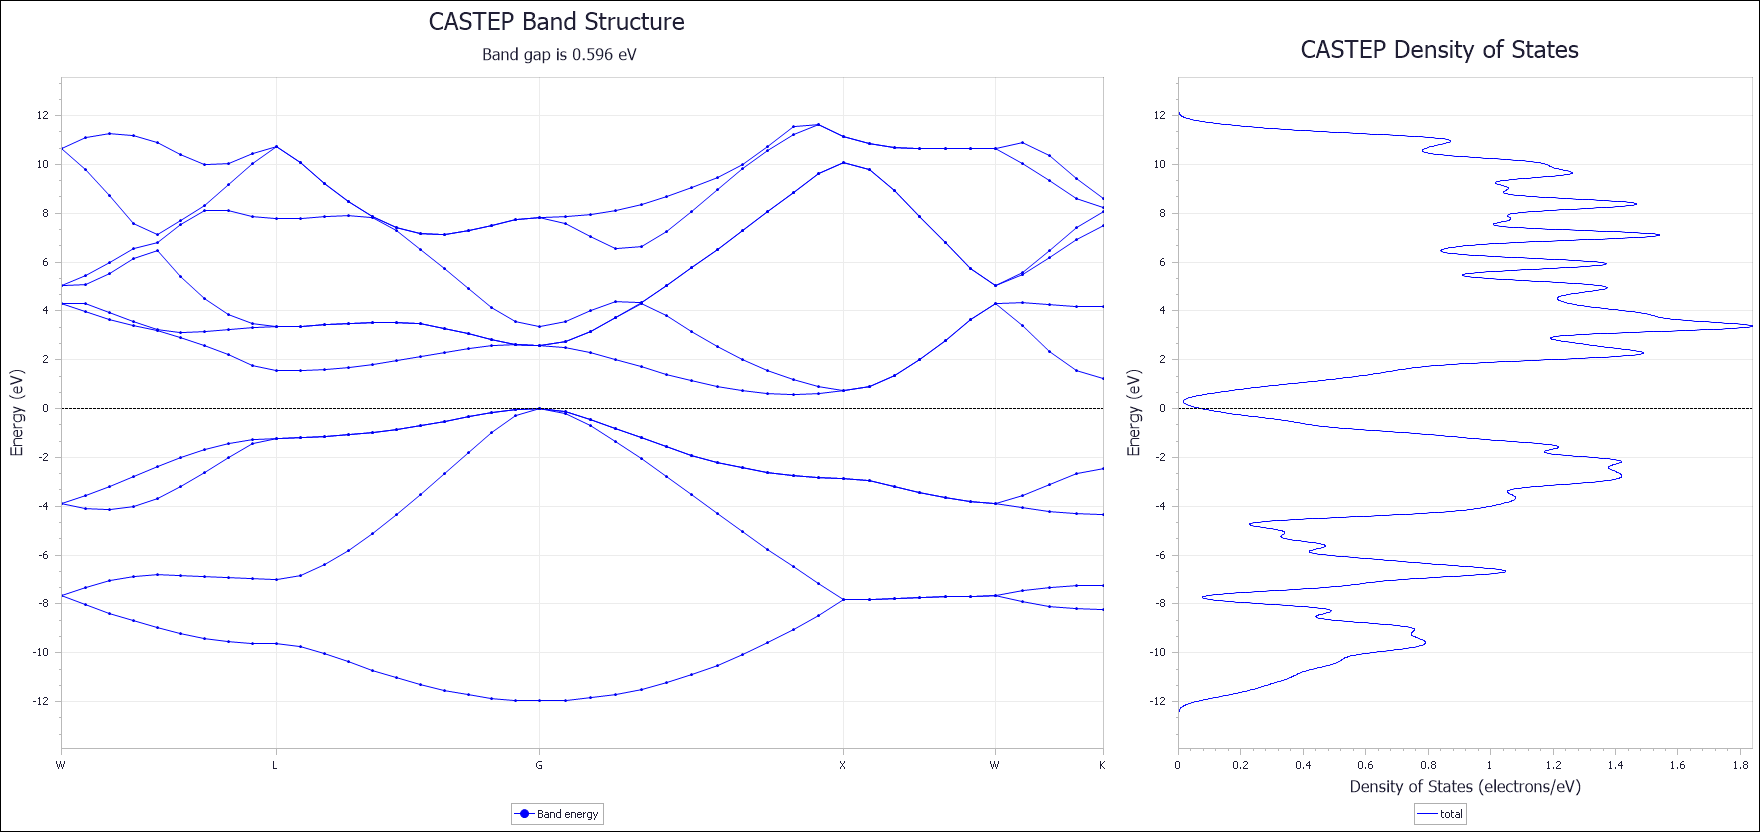
\includegraphics[width=0.9\linewidth]{results/si-band-structure-castep.png}
    \caption{CASTEP 计算的能带结构。}
    \label{fig:si-band-structure-castep}
\end{figure}

\begin{figure}[ht!]
    \centering
    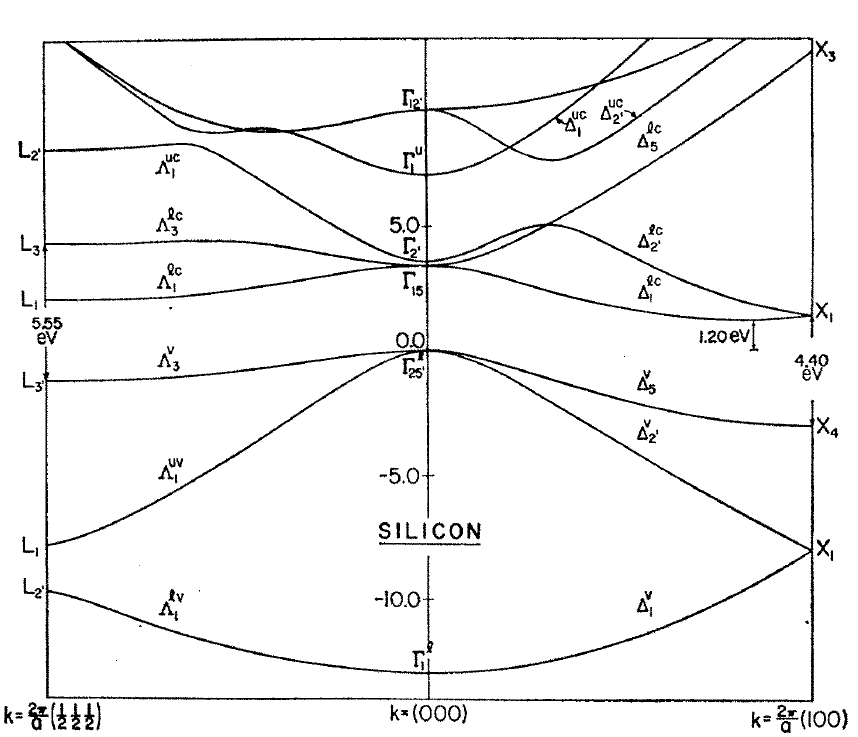
\includegraphics[width=0.6\linewidth]{results/si-band-structure-reference.png}
    \caption{Si 的能带结构,来自 \cite{cardona_energy_band_1966}。}
    \label{fig:si-band-structure-reference}
\end{figure}

与图~\ref{fig:si-band-structure-reference}比较,可见 CASTEP 计算出的能带结构与前人计算的大致相符\cite{phillips_band_1962,cardona_energy_band_1966},但是带隙显著低于测量值($\qty{1.20}{\electronvolt}$左右)。

带隙显著低于测量值是 CASTEP 等使用的密度泛函理论(Density-Functional Theory,DFT)计算的一大特点。
该理论通过计算单一电子加入基态绝缘体系统(即满带)产生的能量变化来求解带隙。
根据定义,带隙的能量为
\begin{equation}
    E_g = (E_{n+1} - E_n) - (E_n - E_{n-1}),
\end{equation}
因此,只要能够准确地计算基态电子的能量,就可以求出带隙的能量。
但是由于电子的交换-相关势能(exchange-correlation potential)在该情况下存在不连续的断点,因此DFT理论无法给出对新增电子的基态能量的准确估计,从而无法给出准确的带隙,这一问题称为“带隙问题”(Band gap problem)\cite{borlido_exchange-correlation_2020,sham_density-functional_1983}。

计算出的声子数据可用于预测材料的热力学数据,如图~\ref{fig:si-thermodynamics}所示。
\begin{figure}
    \centering
    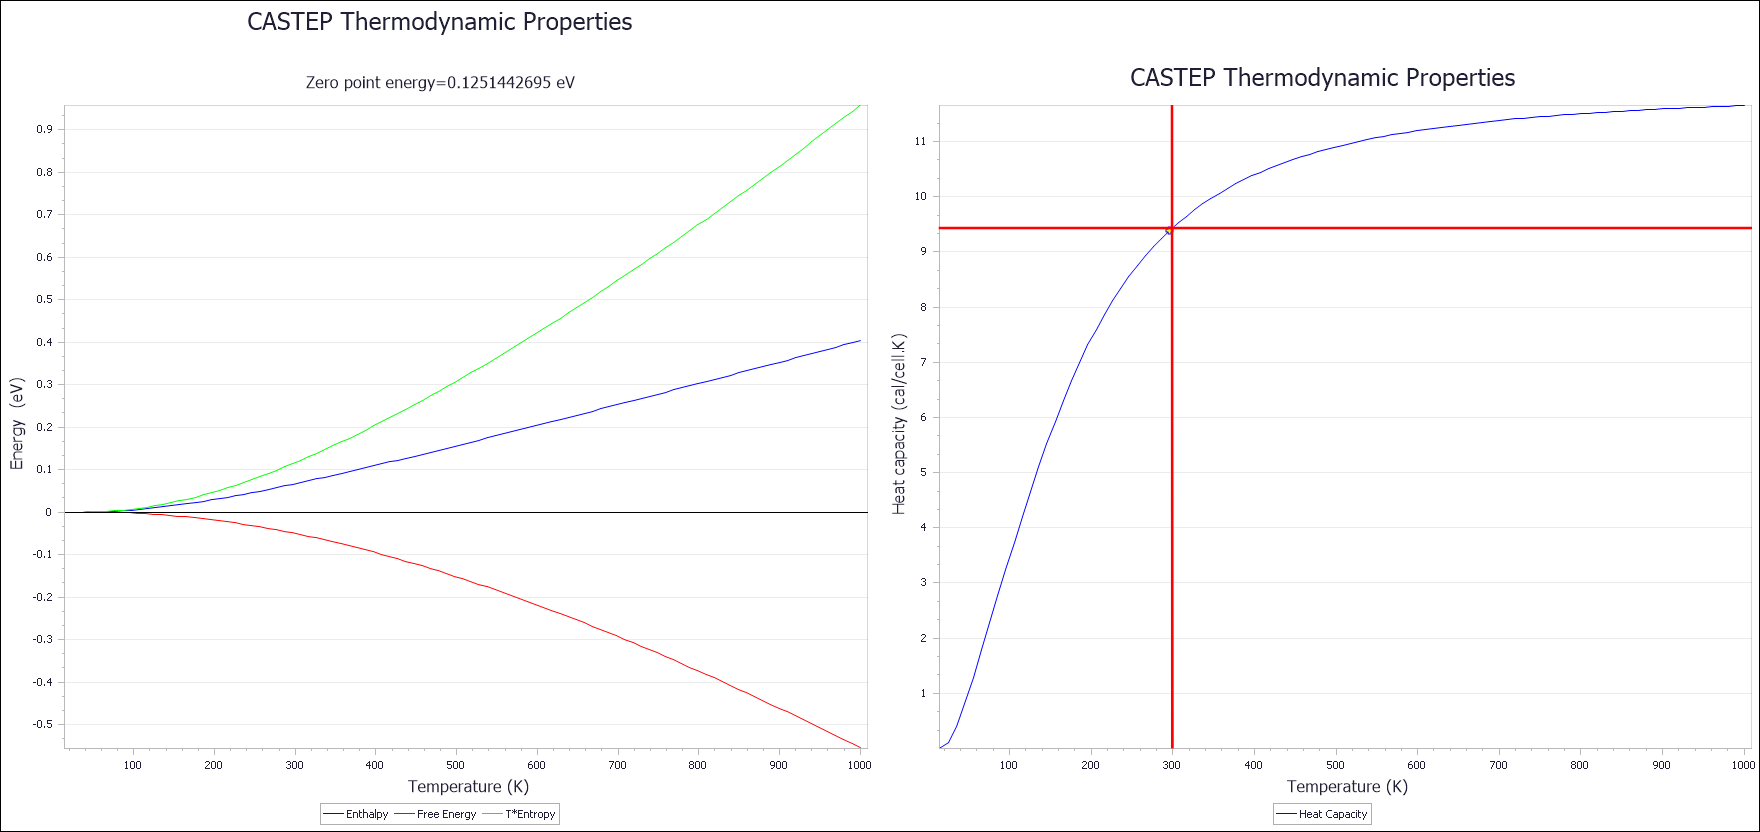
\includegraphics[width=0.8\linewidth]{results/si-thermodynamics.png}
    \caption{CASTEP 预测的热力学数据。}
    \label{fig:si-thermodynamics}
\end{figure}
从图中可读出$\qty{300}{\kelvin}$时比热约为
\begin{equation}
    \qty{9.4}{\calUnit\per\cell\per\kelvin} = 9.4 \times \frac{4.184}{2} \; \unit{\joule\per\mole\per\kelvin} = \qty{19.66}{\joule\per\mole\per\kelvin},
\end{equation}
与实验数据($\qty{20.05}{\joule\per\mole\per\kelvin} \; @ \; \qty{300}{\kelvin}$)较为符合。


\section{结论}
本文回顾了固体物理课程上学习的主要内容,并利用 Material Studio 2020 以及相关的理论武器对硅晶体这一本征半导体的宏观与微观性质进行了预测和验证。
实验说明,固体物理相关的理论是连接物体的宏观与微观性质的桥梁,并且尽管部分数值计算理论在特定的问题上存在缺陷,仍能较好地指导相关的实践活动。

\section{参考文献}
\nocite{*}
\printbibliography[heading=none]

\end{document}
